\documentclass[a4paper]{article}

% French

\usepackage[T1]{fontenc}
\usepackage[french]{babel}
\usepackage[autolanguage]{numprint} % for the \nombre command

\usepackage{graphicx} % images

\usepackage{calc} % Centrer les boites verticalement

\PassOptionsToPackage{hyphens}{url}
\usepackage[]{hyperref}

% \usepackage{breakurl}

\usepackage[lofdepth,lotdepth]{subfig}

% \usepackage{parskip} % // en fin de paragraphe
\usepackage{amsfonts}
\usepackage{amsmath}
\usepackage{wrapfig}

\usepackage{fancyhdr}
  
\usepackage{eurosym}


\usepackage{datetime}
\newdate{date}{01}{04}{2023}
\date{\displaydate{date}}


\newcommand{\modedieu}{\og Mode Dieu \fg}


\title{Analyse d'une fraude facilitée grâce à Fairtiq en Occitanie et Nouvelle-Aquitaine : réflexions sur les conséquences et les solutions possibles}
\author{MALLET Samuel}

\begin{document}
\maketitle

% Configuration - numérotation de page 
\pagestyle{fancy}
\fancyhead{}
\fancyhead[L]{\leftmark}
% \fancyfoot{}
% \fancyfoot[LE,RO]{\thepage} % Left even, right odd


\thispagestyle{empty}

\begin{abstract}
  En 2021, la SNCF a lancé une collaboration avec l'application mobile Fairtiq dans les
  régions Occitanie et Nouvelle-Aquitaine. Cette initiative permet aux voyageurs éligibles
  d'utiliser leur smartphone pour voyager en train TER en appuyant simplement sur un bouton,
  et la facturation du voyage est automatique. Cependant, le billet affiché par l'application
  ne contient pas de code QR ou d'autre moyen de certification, ouvrant ainsi la porte à de
  nombreuses méthodes de fraude potentielles.

  Dans ce document, nous explorons plusieurs techniques de falsification de billets,
  y compris un exemple concret d'application. Nous examinons également comment
  des individus malintentionnés pourraient exploiter ces failles pour en tirer profit,
  notamment à travers diverses arnaques.


\end{abstract}


\begin{figure}[h]
  \includegraphics[width=\textwidth]{illustrations/images/fairtiq_close_up_FR.jpg}
\end{figure}

\clearpage




\section{Introduction}

Je suis un étudiant en double licence mathématiques-informatique de l'université des sciences de Montpellier.
Depuis longtemps, j'ai voulu apprendre à coder des applications et sites web et c'est en 2021 que
j'ai commencé cet apprentissage. Mon objectif est de développer des applications pour divers appareils,
c'est pourquoi je m'intéresse aux frameworks multi-plateformes.
Je réalise quelques projets personnels pour m'exercer, jusqu'au jour
où un employé SNCF me fait découvrir l'application Fairtiq et ses avantages.
Cette application permet de s'affranchir de la réservation des billets de trains, et de pouvoir voyager
grâce à un simple appui sur un bouton.

Lors de ma première utilisation, j'ai remarqué que le billet n'était pas sécurisé
et qu'il serait aisé d'en faire une copie. En effet, n'importe quel développeur web ou mobile pourrait
créer une application ou un site web permettant la configuration et l'affichage d'un faux billet.
Quant à moi, j'étais à la recherche d'un simple projet d'application mobile pour aiguiser mes compétences.
Je me suis alors lancé dans la création d'une application factice.
Il me suffisait de copier l'interface du billet, puis d'ajouter un formulaire permettant d'indiquer
ses informations personnelles nécessaires à l'affichage du billet.
J'ai alors saisi mon nom, mon prénom, ma date de naissance et ma gare de départ (Figure \ref*{sub:first_version:ticket_creation}) et voilà ! J'avais créé
un billet valable sur tout le réseau TER d'Occitanie, parfaitement identique à l'original et pouvant
être présenté aux contrôleurs (Figure \ref*{sub:first_version:ticket_page}). Tout cela a été réalisé dans l'heure suivant ma découverte de Fairtiq.



\begin{figure}
  \begin{center}
    \subfloat[Page de configuration]{
      \includegraphics[width=0.4\textwidth]{illustrations/images/first_version/ticket_creation.jpg}
      \label{sub:first_version:ticket_creation}
    }
    \hspace{0.1\textwidth}
    \subfloat[Page du billet]{
      \includegraphics[width=0.4\textwidth]{illustrations/images/first_version/ticket_page.jpg}
      \label{sub:first_version:ticket_page}
    }
    \caption{Première version de l'application factice}
    \label{fig:first_version}
  \end{center}
\end{figure}



\og Est-ce vraiment aussi simple ? \fg, m'interrogeais-je.
À cet instant, j'ignorais l'âge de l'application et je considérais l'absence de code QR
comme une omission volontaire, due à la jeunesse du système. \og La faille sera corrigée très vite\fg, pensais-je.


J'ai alors mis de côté \og Fairetique\fg\ (le nom que j'avais donné à la fausse application) jusqu'au jour où un
contrôleur a effectué une vérification inhabituelle de mon billet. (J'utilisais bien sûr Fairtiq,
l'application originale, sinon je ne serais pas en train d'écrire ceci, mais plutôt en prison.)
Mon téléphone posé sur la tablette en face de moi,  il l'a tourné vers lui, a quitté l'écran
du billet pour revenir au menu de l'application, puis a affiché à nouveau le billet.
Si j'avais utilisé mon application factice, alors
la supercherie aurait été découverte car le menu principal n'était autre que la page de configuration
du billet (Figure \ref*{sub:first_version:ticket_creation}).
Cette manipulation m'a confirmé que je ne suis certainement pas le seul à avoir \og découvert\fg\ cette faille et apparemment, certains en profiteraient.


J'ai donc décidé de créer une nouvelle version de mon application,
capable de faire face à presque toutes les éventualités et de frauder
sur tous les TER sans limitation.

Pour les lecteurs extérieurs, je commence par une brève présentation de Fairtiq.
Ensuite, je présente quelques méthodes de fraude basées sur l'absence de code QR,
puis je fais une démonstration de mon application factice. Je termine enfin par
une étude des éventuelles conséquences de cette faille.
\clearpage


%================== DISCLAIMER ==================



\begin{center}
  \setlength{\fboxsep}{10pt}
  \vspace*{\fill}

  \fbox{%
    \parbox{0.8\textwidth}{%
      \textbf{Avertissement :}\\[1ex]
      Ce document est rédigé à des fins éducatives et informatives uniquement.
      L'auteur ne promeut ni n'encourage la fraude ou toute autre activité illégale.
      Les exemples et méthodes décrits ici sont destinés à sensibiliser les
      lecteurs aux risques potentiels liés à l'absence de code QR sur les billets
      de train et à encourager l'amélioration de la sécurité des systèmes de
      billetterie. En aucun cas, l'auteur ne saurait être tenu responsable
      de l'utilisation abusive des informations contenues dans ce document.
    }
  }
  \vspace*{\fill}
\end{center}



\clearpage

\tableofcontents

\clearpage


\section{Qu'est-ce que Fairtiq ?}



Fairtiq est une application pour smartphones simplifiant l'achat de billets pour les transports en commun.
\href{https://fairtiq.com/fr}{Le site de la marque} indique : \og D’un geste, obtenez le bon billet, toujours au prix le plus optimal \fg.

\subsection{Utilisation}
Le principe de Fairtiq est simple : après avoir configuré l'application, celle-ci géolocalise l'utilisateur.
Lorsqu'il est détecté dans une gare ou une station de train, il suffit de faire glisser le bouton "start"
pour débuter le trajet (Figure~\ref{sub:start_button}).

Grâce au GPS du smartphone,
l'application détermine automatiquement le trajet effectué par l'utilisateur.

À la fin du voyage, il suffit d'appuyer de nouveau sur le même bouton pour mettre fin au trajet (Figure~\ref{sub:stop_button}). Le trajet est ensuite calculé et facturé automatiquement à l'utilisateur.



\begin{figure}[h]
  \begin{center}
    \subfloat[Billet non démarré]{
      \includegraphics[width=0.4\textwidth]{illustrations/images/start_button.png}
      \label{sub:start_button}
    }
    \hspace{0.1\textwidth}
    \subfloat[Billet démarré]{
      \includegraphics[width=0.4\textwidth]{illustrations/images/stop_button.jpg}
      \label{sub:stop_button}
    }
    \caption{Captures d'écran de Fairtiq dans une gare}
    \label{fig:start_stop_buttons}
  \end{center}
\end{figure}

\clearpage
\subsection{Le billet}

Lors d'un contrôle, le voyageur affiche son billet grâce au bouton \og \textit{Afficher mon billet}\fg\
visible sur la figure~\ref*{sub:stop_button}.

Ce billet contient :
\begin{itemize}
  \item Un chronomètre indiquant le temps écoulé depuis l'activation du billet,
        permettant de vérifier que le voyageur ne l'a pas activé juste avant l'arrivée du contrôleur.
  \item La gare ou l'arrêt de départ.
  \item Le nom et la date de naissance du voyageur
  \item Des informations supplémentaires propres à la compagnie de transport.
\end{itemize}

On pourrait s'attendre à ce que ce billet inclut également un code QR,
ce qui est effectivement le cas pour certaines compagnies de transport en Suisse
et en Allemagne (Figure \ref{sub:billet_avec_qr_2}).
De plus, lors du téléchargement de Fairtiq depuis les magasins d'applications
App Store et Play Store, l'une des images d'illustration présente un
billet contenant un code QR (Figure \ref*{sub:billet_avec_qr_1}).


\begin{figure}[h]
  \begin{center}
    \subfloat[Source : \textit{Play Store}]{
      \includegraphics[height=8cm]{illustrations/images/billet_avec_qr_1.jpg}
      \label{sub:billet_avec_qr_1}
    }
    \hspace{0.1\textwidth}
    \subfloat[Source : \textit{stwab.de}]{
      \includegraphics[height=8cm]{illustrations/images/billet_avec_qr_2.jpg}
      \label{sub:billet_avec_qr_2}
    }
    \caption{Billets numériques avec code QR}
    \label{fig:billets_avec_qr}
  \end{center}
\end{figure}


\vspace*{1cm}

\clearpage



\subsection{Fairtiq et la SNCF}
Depuis 2016, Fairtiq s'est progressivement implantée en Suisse, au Liechtenstein,
en Autriche, en Allemagne et en Belgique (dans cet ordre) (Figure \ref*{fig:rayon_validite}).
C'est en 2021 \cite{fairtiq-fete-ses-5-ans}
qu'elle arrive en France en partenariat avec la SNCF
et dans les régions Occitanie et Nouvelle-Aquitanie. Ces dernières promettent une expérience utilisateur
simplifiée ainsi qu'une réduction du coût des trajets et ce pour tous les trains \textit{TER}.

\begin{figure}
  \centering
  \includegraphics[width=\textwidth]{illustrations/images/rayon_validite_fairtiq.png}
  \caption{\centering Rayon de validité de Fairtiq (\textit{fairtiq.com})}
  \label{fig:rayon_validite}
\end{figure}


\subsubsection{Fairtiq en Occitanie}
\paragraph{Pour les jeunes : }

Lancée en avril 2021, l'offre \og $+=0$\fg\ de l'Occitanie a d'abord été testée sur un panel de 2000 jeunes entre 18 et 26 ans.
C'est en septembre qu'elle fut rendue disponible à l'ensemble les jeunes de cette tranche
d'âge.  Cette offre leur permet de ne pas payer plus de 50\% du prix des trajets,
voire de voyager gratuitement en fonction du nombre de trajets effectués.
Les détails de l'offre décrits en figure \ref*{fig:plus_eq_zero} indiquent qu'un voyageur effectuant
au moins 15 allers-retours par mois peut donc voyager gratuitement. En revanche, si ce voyageur est moins régulier
et effectue moins de 15 allers-retours par mois, il voyage gratuitement à partir du 11$^{e}$ trajet, mais
devra régler une partie ou la totalité de ses 10 premiers trajets du
mois suivant \cite{plus_eq_zero}.

\begin{figure}
  \centering
  \includegraphics[width=\textwidth]{illustrations/images/offres/occitanie/plus_eq_zero.jpg}
  \caption{L'offre +=0 de la région Occitanie}
  \label{fig:plus_eq_zero}
\end{figure}


Récemment, il a été annoncé que, dès septembre 2023, ce dispositif serait étendu aux jeunes
dès 16 ans ainsi qu'aux lignes régulières du réseau liO autocars pour les
18-26 ans \cite{nouvelle-convention}.



\paragraph{Pour les séniors : }
Destinée aux personnes âgées de 60 ans et plus, l'offre \og +=- \fg\ est apparue plus d'un an plus après l'offre prédédente,
proposant des réductions allant de -10\% à -50\%, détaillées en figure \ref*{fig:plus_eq_moins}
\cite{plus_eq_moins}.

\begin{figure}
  \centering
  \includegraphics[width=\textwidth]{illustrations/images/offres/occitanie/plus_egal_moins/reductions.jpg}
  \caption{L'offre +=- de la région Occitanie \cite{plus_eq_moins}}
  \label{fig:plus_eq_moins}
\end{figure}

\paragraph{}
Les jeunes comme les séniors bénéficient alors de tous les trains \og liO \fg\ d'Occitanie, sur plus de 30 lignes
et 280 gares (Figure \ref*{fig:map_occitanie}) \cite{stats-ter-occitanie}.


\begin{figure}
  \centering
  \includegraphics[width=\textwidth]{illustrations/images/offres/occitanie/reseau_ferroviaire_occitanie.png}
  \caption{Le réseau ferroviaire régional d'Occitanie (\textit{ter.sncf.com})}
  \label{fig:map_occitanie}
\end{figure}


\clearpage

\subsubsection{Fairtiq en Nouvelle-Aquitaine}
Similairement, la région Nouvelle-Aquitaine a instauré une offre pour ses TER
en recourant à l'application Fairtiq. Baptisée \og FlexTER\fg\, elle était initialement réservée aux moins de 28 ans
mais elle est accessible à tous depuis le mois d'avril 2022 \cite{extention-toute-nouvelle-aquitaine}.

Contrairement aux offres de l'Occitanie, les réductions appliquées ne sont pas spécifiques à Fairtiq,
mais dépendent des autres offres et abonnements de la région. Le calcul de la facturation s'effectue chaque semaine,
et détermine l'offre la plus avantageuse pour le voyageur.

Cela garantit que l'utilisateur ne paiera pas plus cher ses trajets en passant par
Fairtiq que s'il avait souscrit à un abonnement par lui-même, et tout cela est sans engagement \cite{flexter}.
Les utilisateurs peuvent voyager sur tout le réseau de TER de la Nouvelle-Aquitaine, représenté
en figure \ref*{fig:map_nouvelle_aquitaine}.


\begin{figure}
  \centering
  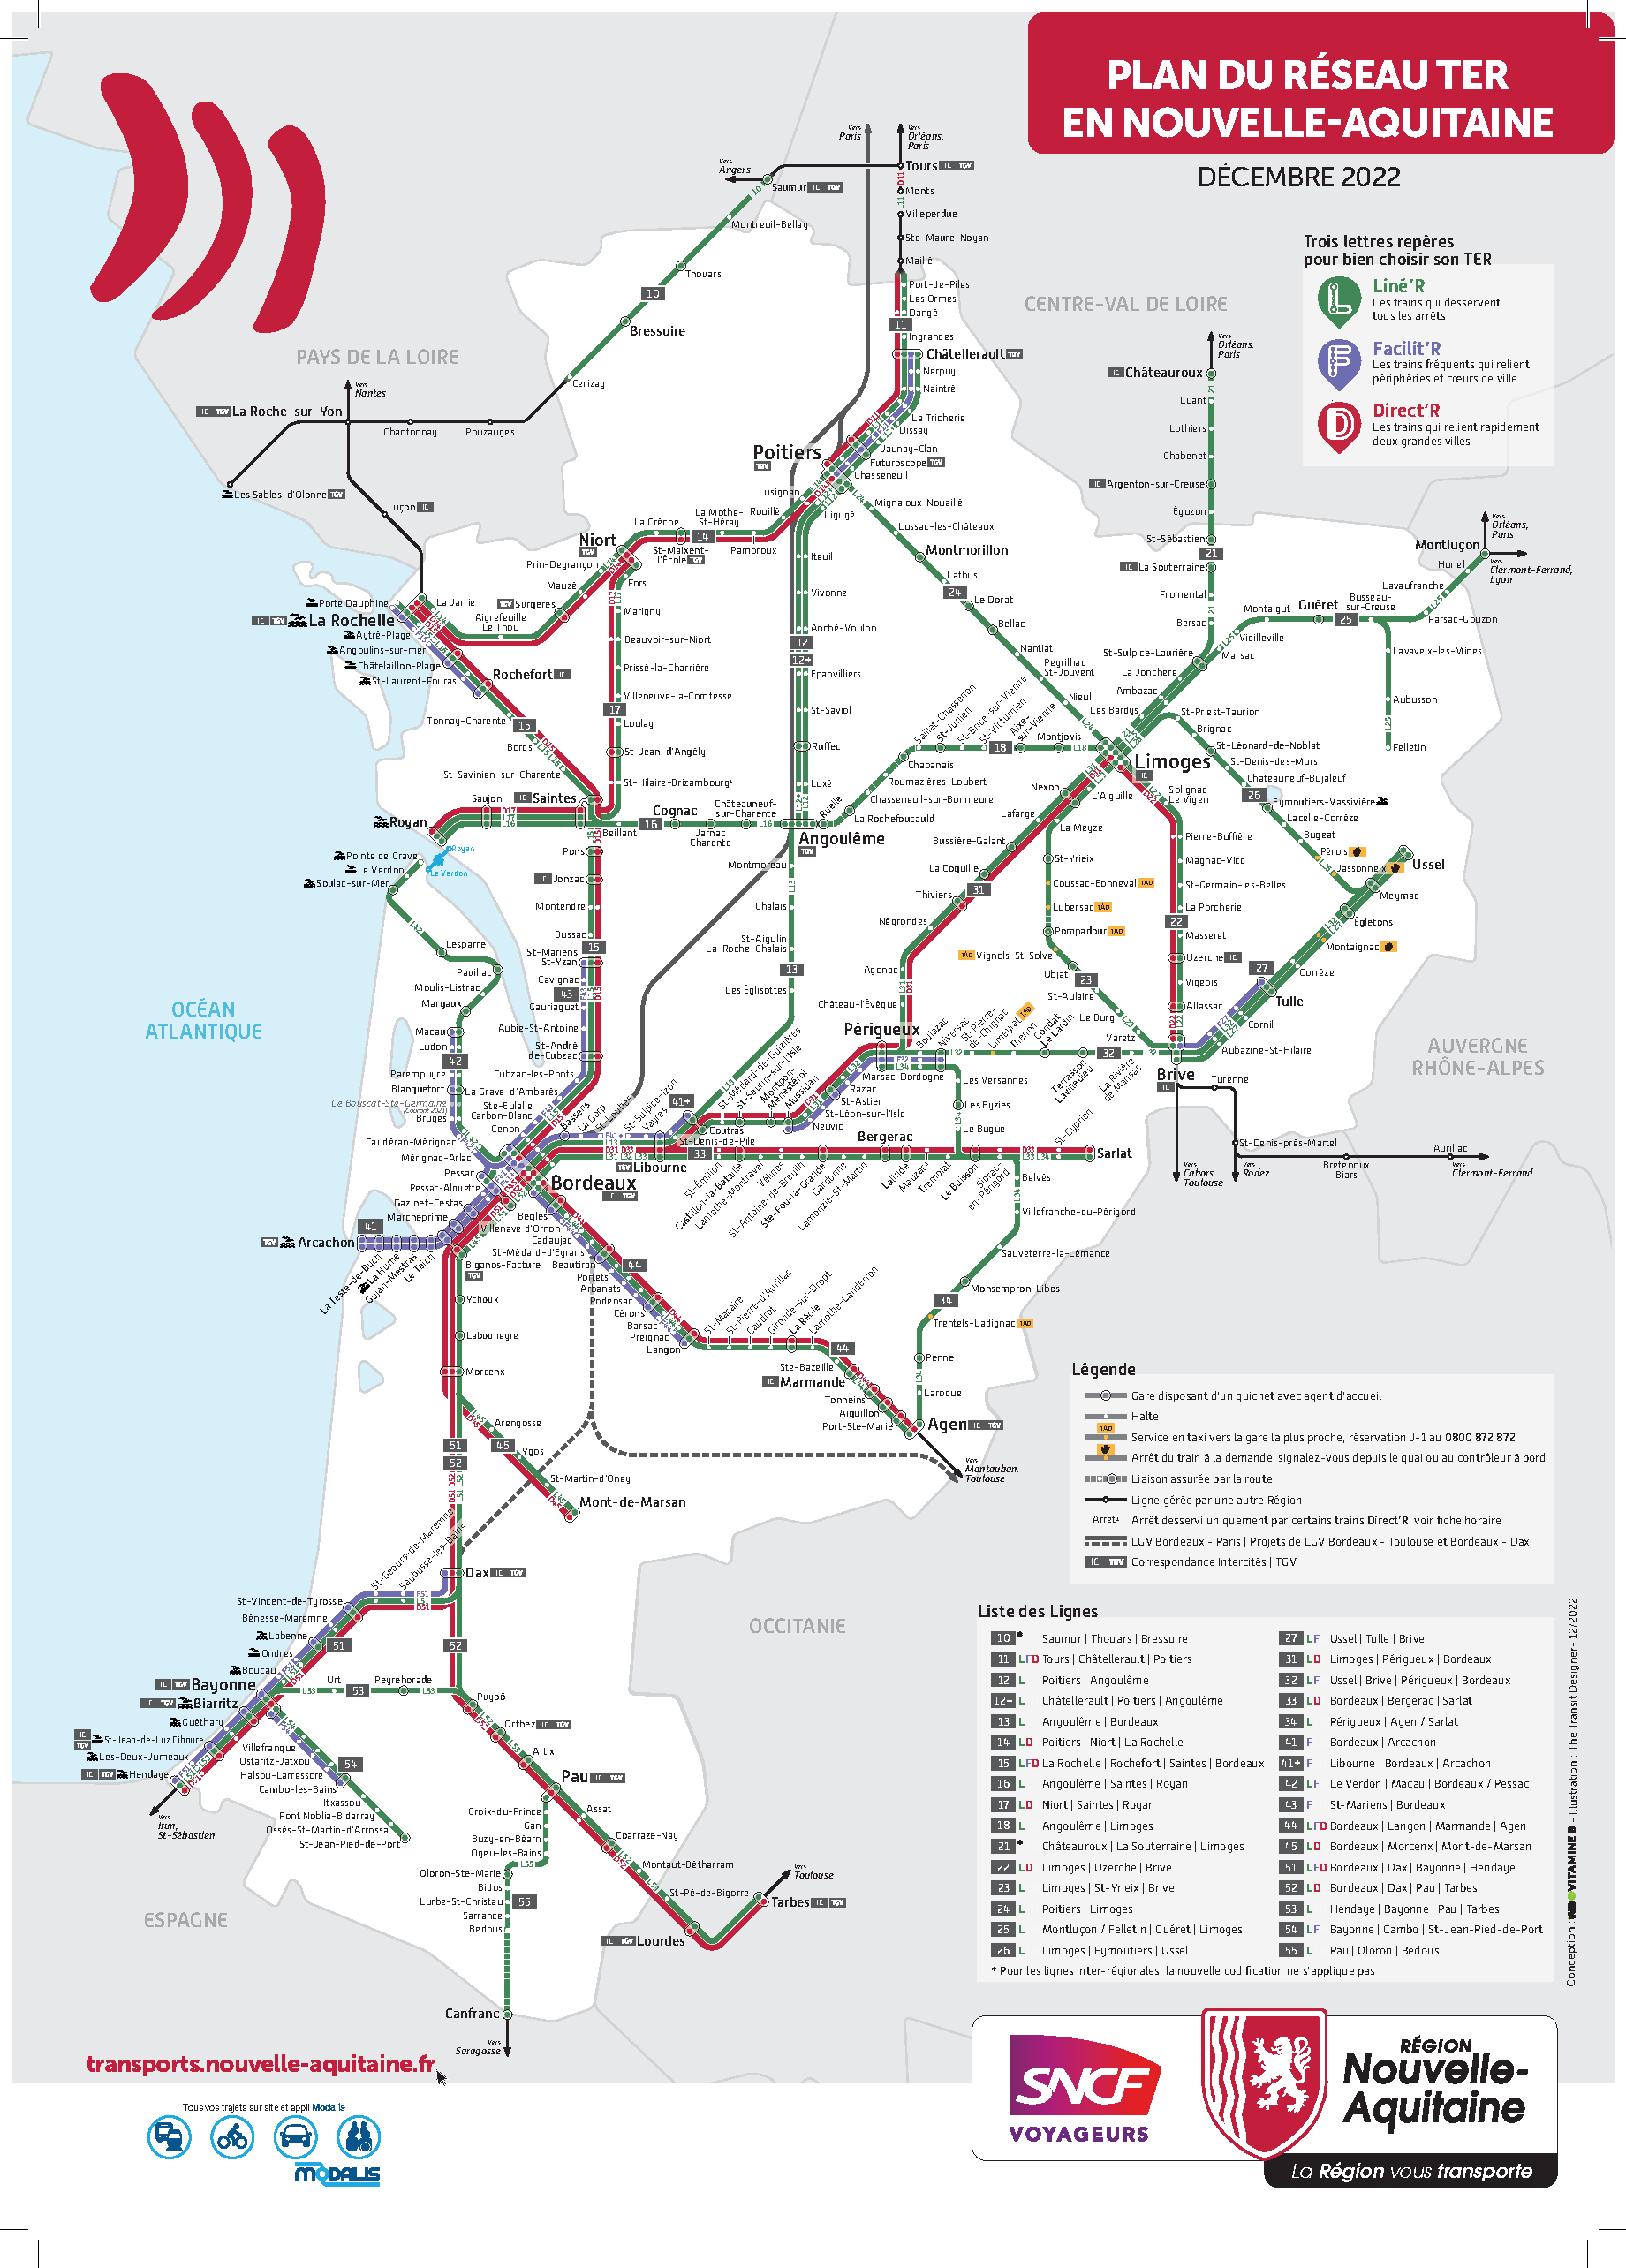
\includegraphics[width=\textwidth]{illustrations/images/offres/nouvelle-aquitaine/carte_reseau.png}
  \caption{\centering Le réseau ferroviaire régional de la Nouvelle Aquitaine (\textit{ter.sncf.com})}
  \label{fig:map_nouvelle_aquitaine}
\end{figure}

\clearpage
\subsubsection{Voyage interrégional}
Nous avons vu précédemment que Fairtiq est disponible pour les jeunes et les seniors à
la fois en Occitanie et en Nouvelle-Aquitaine.
Mais est-il possible de voyager d'une région à l'autre sans friction ?


Il est intéressant de noter que certaines gares situées en Nouvelle-Aquitaine,
comme celles de Pau, Agen et Brive-la-Gaillarde, sont accessibles depuis le réseau Occitan.
Cela est visible sur la carte de la figure \ref*{fig:map_occitanie}.
Une fois dans l'une de ces gares, il suffit à l'utilisateur de se rendre sur l'application Fairtiq et
de changer de région active (Figure \ref*{fig:changement_region})
pour continuer son trajet dans toute la Nouvelle-Aquitaine.
Bien que cette méthode puisse prendre un peu plus de temps, il est possible d'effectuer un trajet comme Perpignan-Poitiers (et inversement) en utilisant uniquement les TER et l'application Fairtiq.


\begin{figure}[h]
  \centering
  \includegraphics[width=\textwidth]{illustrations/images/changement_regions/changement_illustration.png}
  \caption{Changement de la région dans Fairtiq}
  \label{fig:changement_region}
\end{figure}





\clearpage

\section{De nouvelles méthodes de fraude}

\textit{Dorénavant, nous évoquerons Fairtiq uniquement pour une utilisation dans les régions Occitanie et Nouvelle-Aquitaine.}


Bien que cette application simplifie grandement l'achat de billets, elle ouvre la voie à de nouvelles méthodes de fraude.
Déjà, rien n'empêche un voyageur qui effectue un trajet en train d'arrêter son billet juste après un contrôle,
afin d'effectuer la fin de son trajet gratuitement.

Cependant, Fairtiq pourrait continuer d'analyser le comportement de l'utilisateur après l'arrêt du billet, afin de
détecter cette manipulation \cite{stop-billet-avant-descente}.
Pour s'en prémunir, un utilisateur pourrait couper le GPS du smartphone et arrêter complètement Fairtiq pour l'empêcher de fontionner en arrière plan.
De cette manière, Fairtiq ne serait pas en mesure de déterminer si l'utilisateur a continué son trajet dans le train après l'arrêt du billet.

Il est à noter qu'une méthode similaire existe en utilisant des application classiques de billeterie, bien que cela soit plus difficile.
Par exemple, un voyageur effectuant un trajet direct de Toulouse à Montpellier pourrait dans un premier temps réserver un billet
Toulouse-Carcasonne. S'il n'est pas contrôlé lors de cette première partie, alors il achete un billet Carcassone-Montpellier.
Ceci peut être réalisé notamment grâce à l'application SNCF Connect, qui permet de réserver des billets de TER quelques minutes avant le départ
de la gare concernée. En admettant que l'utilisateur ait une chance sur deux d'être contrôlé lors de la première partie de son trajet,
il a alors une chance sur deux de diviser le coût de son trajet par deux. En moyenne, cela fait donc une réduction de 25\% du coût total des trajets.

En raison de la possibilité d'arrêter son trajet à tout moment lors d'un voyage avec Fairtiq, il est bien plus facile
et efficace d'effectuer cette manipulation avec cette application.  Cet incovénient est donc causé par un des plus grands
avantages de l'application, et cela semble difficile à surmonter.

En revanche, les méthodes suivantes exploitent l'absence de certification du billet Fairtiq,
qui se limite à afficher la date, l'heure, le nom et la date de naissance de l'utilisateur,
ainsi que la gare de montée. Il est donc impossible de vérifier l'authenticité
d'un billet sans informations supplémentaires. Il suffit en effet d'imiter le billet,
ce que les sections suivantes décrivent en détail.


\subsection{Capture d'écran du billet}
Puisqu'il est désormais très facile de faire une capture vidéo de l'écran de son smartphone,
un utilisateur qui effectue souvent le même trajet pourrait être tenté d'effectuer une
capture vidéo de son billet durant une partie ou la totalité du son voyage.
Ainsi, lors de ses prochains trajets, il pourrait présenter la vidéo au contrôleur.

Cependant, cette technique n'est pas infaillible, car chaque billet incorpore la date et l'heure du trajet.
Puisque ces informations sont relativement petites, l'individu pourrait espérer qu'elles passent inaperçues. De plus,
il pourrait diminuer la taille des polices de son smartphone pour rendre le billet plus difficile à lire.


\subsection{Montage vidéo}
Pour régler le problème de la date, un individu ayant des compétences de base en montage
vidéo pourrait facilement modifier la date sur la capture d'écran avant son trajet.
En changeant également le texte indiquant la gare de départ ainsi que le le chronomètre,
il serait possible de générer la vidéo d'un billet pour n'importe quel trajet.
Il n'est pas difficile d'imaginer que le processus pourrait être automatisé, ou au moins
accéléré, rendant possible la génération d'un billet peu de temps avant chaque trajet.

Cependant, bien que cela semble rare, le contrôleur serait en mesure de demander à
voir d'autres éléments de l'application s'il le jugeait nécessaire. Par exemple,
demander à quitter la page du billet pour retourner à l'accueil de l'application,
comme je l'ai décrit dans l'introduction. Ce désagrément peut être prévenu en
créant une copie presque parfaite de l'application.


\clearpage

\section{Un exemple d'application factice}

Je présente dans cette section un exemple d'application
permettant d'afficher un faux billet tout en imitant parfaitemant l'interface
de Fairtiq.

En plus de devoir répondre aux défis déjà abordés, l'application doit également être facile
à utiliser, car nous considérons qu'elle pourra être rendue publique. Cette précision sera utile
dans la section \ref*{sec:consequences}.

\subsection{Première utilisation}
Lors de la première ouverture de l'application, l'utilisateur est présenté à une brève introduction à
Fairtiq et à \og Fairetique \fg\ (Figure \ref*{fig:fairetique_intro}). Il est en effet essentiel
que l'utilisateur soit informé du fonctionnement normal de Fairtiq.

Bien que le slogan \og Voyagez, ne payez plus \fg\ manque d'originalité,
il décrit parfaitement ce à quoi l'utilisateur doit s'attendre.
Toutefois, l'application avertit l'utilisateur de l'illégalité de son acte et
impose la coche d'une case (Figure \ref*{sub:intro_tuto_fairetique_disclaimer}).


\begin{figure}[h]
  \begin{center}
    \subfloat[Introduction]{
      \includegraphics[width=0.32\textwidth]{illustrations/images/intro/slogan.jpg}
      \label{sub:intro_slogan}
    }
    % \hspace{0.1\textwidth}
    \subfloat[Fonctionnement de Fairtiq]{
      \includegraphics[width=0.32\textwidth]{illustrations/images/intro/tuto_fairtiq_sliding.jpg}
      \label{sub:intro_tuto_fairtiq}
    }
    % \hspace{0.1\textwidth}
    \subfloat[\centering Fonctionnement de \og Fairetique\fg]{
      \includegraphics[width=0.32\textwidth]{illustrations/images/intro/tuto_fairetique_disclaimer.jpg}
      \label{sub:intro_tuto_fairetique_disclaimer}
    }
    \caption{Première ouverture de l'application factice}
    \label{fig:fairetique_intro}
  \end{center}
\end{figure}



Après cette brève introduction, l'application demande à l'utilisateur d'entrer son nom,
son prénom et sa date de naissance (Figure \ref*{sub:user_profile_creation}).
Ces informations seront nécessaires à l'affichage du billet.

Ensuite, l'utilisateur est invité à autoriser (ou non) l'utilisation du GPS, et est
ensuite redirigé vers la page d'accueil.

Enfin, une fois la configuration terminée, l'application peut être
utilisée de façon indistinguable de l'application originale.

Lorsque l'utilisateur ouvre l'application, il est automatiquement géolocalisé
et la gare la plus proche est sélectionnée comme gare de départ. Ensuite,
l'utilisateur peut démarrer et afficher le billet (Figure \ref*{sub:fake_homepage}).

\begin{figure}
  \begin{center}
    \subfloat[Configuration]{
      \includegraphics[width=0.4\textwidth]{illustrations/images/user_profile_creation.jpg}
      \label{sub:user_profile_creation}
    }
    \hspace{0.1\textwidth}
    \subfloat[Page d'accueil]{
      \includegraphics[width=0.4\textwidth]{illustrations/images/fake_homepage.jpg}
      \label{sub:fake_homepage}
    }
    \caption{Captures d'écran de l'application factice}
  \end{center}
\end{figure}

\clearpage

\subsection{Activation d'un faux billet}
Le billet se démarre exactement comme l'a montré la figure \ref{fig:start_stop_buttons}.
Ensuite, même si l'application est fermée, ou que le l'appareil n'a plus de batterie, le billet restera encore
actif à la réouverture (sauf exception, voir section \ref*{sssec:desactivation_billet_auto}).

L'utilisateur peut ensuite afficher son faux billet (Figure \ref{fig:ticket_generation}).

\begin{figure}[hb]
  \centering
  \includegraphics[width=0.6\textwidth]{illustrations/images/ticket_generation/ticket_generation.png}
  \caption{Génération du billet }
  \label{fig:ticket_generation}
\end{figure}

\hspace{1cm}

\begin{wrapfigure}{r}{0.6\textwidth}
  \centering
  \includegraphics[width=0.3\textwidth]{illustrations/images/no-gps/acces_restreint_position.jpg}
  \caption{Avertissement GPS indisponible}
  \label{fig:no-gps-alert2}
\end{wrapfigure}

Si l'application n'a pas accès au GPS, ou que celui-ci est désactivé,
l'avertissement affiché est identique à l'original (Figure \ref{fig:no-gps-alert2}).

Nous verrons plus loin qu'il est possible de passer outre cette alerte si l'utilisateur souhaite
tout de même utiliser l'application sans GPS (voir section \ref*{sssec:no_gps_usage}).


\clearpage

\subsection{Le \modedieu}
Maintenant qu'il est possible de générer un faux billet, il reste des problèmes à surmonter.

D'abord, voyons l'exemple d'un individu qui utilise la fausse application, et qui se rend compte
une fois dans le train qu'il a oublié d'activer son billet. Il active alors son billet
immédiatement, ce qui est toujours possible même loin d'une gare. Le problème survient
lorsque cela fait plusieurs minutes que le train ne s'est pas
arrêté à une gare, et que le billet affirme qu'il est activé depuis seulement quelques minutes.
Un contrôleur pourrait déceler un problème, car Fairtiq \textit{original} rend impossible l'activation
du billet entre deux gares.\par
De plus, un contrôleur pourrait penser que le voyageur a tenté de frauder en activant
son billet juste avant le contrôle.

Pire encore, l'application pourrait localiser l'utilisateur à la prochaine gare, s'il sagit de la
gare la plus proche. On pourrait alors penser à calculer le sens de déplacement de l'utilisateur et veiller à
affecter la gare de départ à une gare de laquelle il s'éloigne. Bien que cela marcherait dans le cas
décrit ci-dessus, un utilisateur qui active son billet pendant qu'il se rend en voiture
à sa gare de départ sera localisé à la gare la plus proche parmi les gares derrière lui,
ce qui est indésirable.

Enfin, dans le cas où le GPS serait désactivé ou indisponible, il sera alors impossible de
localiser la gare de départ.

Il devient alors nécessaire d'implémenter un moyen de changer l'heure d'activation du billet,
ainsi que la gare de départ. C'est pourquoi nous introduisons le \textbf{\modedieu}.


\begin{figure}[h]
  \centering
  \includegraphics[width=0.75\textwidth]{illustrations/images/mode_dieu/ouverture_mode_dieu.png}
  \caption{Ouverture du \modedieu}
  \label{fig:ouverture_mode_dieu}
\end{figure}


Ce menu caché s'ouvre d'un appui long sur logo Fairtiq de la page d'accueil (Figure \ref*{fig:ouverture_mode_dieu}).
Fait pour ne pas s'ouvrir accidentellement, il se ferme automatiquement à la réouverture de l'application
afin de rendre l'application utilisable sous les yeux d'un contrôleur. Toutes sortes de configurations
deviennent alors possible, et les principales sont passées en revue ci-dessous.



\subsubsection{Changement de la gare de départ}

À tout moment, l'utilisateur peut changer sa gare de départ : en la cherchant parmi une longue liste,
ou alors en utilisant la barre de recherche (Figure \ref{sub:edit_station}). Il est également
possible de laisser l'application afficher les gares les plus proches (Figure \ref{sub:edit_station_geo}).

Cela protège l'utilisateur de tout problème de GPS et il devient alors possible de rétablir sa gare
de départ lors d'une erreur de localisation (par exemple lors d'une activation tardive du billet).


\begin{figure}[h]
  \begin{center}
    \subfloat[]{
      \includegraphics[width=0.4\textwidth]{illustrations/images/mode_dieu/edit_station/edit_station.jpg}
      \label{sub:edit_station}
    }
    \hspace{0.1\textwidth}
    \subfloat[]{
      \includegraphics[width=0.4\textwidth]{illustrations/images/mode_dieu/edit_station/edit_station_geo.jpg}
      \label{sub:edit_station_geo}
    }
    \caption{Modification de la gare de départ}
  \end{center}
\end{figure}

\clearpage

\subsubsection{Changement de l'heure d'activation du billet}

\begin{wrapfigure}{r}{0.4\textwidth}
  \begin{center}
    \includegraphics[width=0.38\textwidth]{illustrations/images/mode_dieu/votre_billet/votre_billet.jpg}
  \end{center}
  \caption{\centering Modification du billet}
  \label{fig:votre_billet}
\end{wrapfigure}

Dans le cas où l'utilisateur active en retard son billet ainsi que dans une multitude d'autres situations similaires,
l'utilisateur a alors la possiblité de modifier l'heure d'activation afin de la faire correspondre à une situation légitime.
Il peut choisir une nouvelle heure d'activation, ou simplement ajouter ou retirer du temps à la durée
du billet (Figure \ref{fig:votre_billet}).

Par ailleurs, cette date est toujours stockée dans la mémoire permanente du smartphone
et il n'y a donc aucun décalage lorsque l'application est fermée ou lorsque le téléphone éteint.
\subsubsection{Désactivation du billet automatique} \label{sssec:desactivation_billet_auto}
Dans l'application officielle, l'utilisateur doit signaler manuellement sa descente du
train afin que l'application puisse arrêter le billet à temps. Toutefois, il est
également possible d'activer la fonctionnalité \og Smart Stop\fg, qui prend en charge cette
opération de manière automatique. Cependant, avec notre application frauduleuse,
il est facile d'oublier de désactiver le billet, ce qui peut poser problème lors
de voyages ultérieurs.  Par exemple, il est possible lors de l'ouverture de
l'application que le billet précédent soit
toujours actif, ce qui représente un risque en cas de contrôle à la montée.

Pour éviter cela, l'application frauduleuse permet à l'utilisateur de configurer un
délai d'expiration, au-delà duquel le billet est automatiquement désactivé (Figure \ref*{fig:auto_stop}).


\begin{figure}[h]
  \includegraphics[width=0.6\textwidth]{illustrations/images/mode_dieu/auto_stop.jpg}
  \centering
  \caption{Paramètre de l'arrêt automatique du billet}
  \label{fig:auto_stop}
\end{figure}

\subsubsection{Usage sans GPS} \label{sssec:no_gps_usage}


\begin{wrapfigure}{r}{0.5\textwidth}
  \begin{center}
    \includegraphics[width=0.43\textwidth]{illustrations/images/no-gps/discard_alert.jpg}
  \end{center}
  \caption{Paramètre de l'alerte GPS}
  \label{fig:discard_alert}
\end{wrapfigure}

Nous avons vu précédemment (Figure \ref{fig:no-gps-alert2}) qu'une alerte est affichée lorsque
le GPS n'est pas disponible. Dans ce cas, il n'est pas possible de démarrer son billet à moins de passer
par le \modedieu. On laisse alors le choix à l'utilisateur de ne plus afficher cette alerte,
ce qui changera les textes indiquant la gare de départ par des icônes de chargement (Figure \ref*{fig:discard_alert}).
L'utilisateur sera alors libre de la sélectionner manuellement en passant par le \modedieu.

\subsubsection{Guidage de l'utilisateur}
Après l'installation et une fois que l'utilisateur a renseigné les informations nécessaires pour le billet,
un message s'affiche pour indiquer comment accéder au \modedieu.
L'utilisateur peut choisir d'ignorer immédiatement ce message et de lancer un billet ou de suivre
l'indication pour ouvrir le menu caché.

Lors de la première ouverture du menu, l'application guide l'utilisateur dans l'exploration de toutes les fonctionnalités cachées.
Cet accompagnement doit pouvoir être terminé en une minute.
Trois exemples sont illustrés dans la figure \ref*{fig:god_mode_guide}.


\begin{figure}[hb]
  \begin{center}
    \subfloat{
      \includegraphics[width=0.30\textwidth]{illustrations/images/guidage_mode_dieu/open_god_mode.jpg}
      \label{sub:guide_open_gode_mode}
    }
    \subfloat{
      \includegraphics[width=0.30\textwidth]{illustrations/images/guidage_mode_dieu/welcome_god_mode.jpg}
      \label{sub:guide_welcome_god_mode}
    }
    \subfloat{
      \includegraphics[width=0.30\textwidth]{illustrations/images/guidage_mode_dieu/departure_station.jpg}
      \label{sub:guide_departure_station}
    }
    \caption{\centering Présentation du \og Mode dieu \fg\ à l'utilisateur \textit{(non exhaustif)}}
    \label{fig:god_mode_guide}
  \end{center}
\end{figure}

% ===============


\clearpage



\subsection{Détails techniques}
\paragraph*{Accès à l'application - }
Cette application est entièrement réalisée à l'aide du framework
Flutter\footnote{Flutter est un kit de développement logiciel (SDK)
  d'interface utilisateur open-source créé par Google. Il est utilisé
  pour développer des applications pour Android, iOS, Linux, Mac, Windows,
  Google Fuchsia et le web à partir d'une seule base de code. (\textit{flutter.dev})}.
Ainsi, l'application peut être exportée pour les appareils Android et
iOS, ainsi que pour les navigateurs web.

Bien qu'elle puisse être facilement installée et partagée sur Android via un fichier \textit{.apk},
cela est plus difficile pour les appareils Apple. En effet, la marque rend impossible, ou très difficile
l'installation d'applications inconnues, sans passer par le magasin officiel \og App Store \fg. Alors
une solution serait d'héberger l'application sur un serveur web afin la rendre accessible depuis un navigateur.
Cela peut être fait localement : en connectant son ordinateur au même réseau wifi que son smartphone -
par exemple grâce à un partage de connexion initié sur l'appareil mobile - puis en hébergeant l'application
sur l'ordinateur. Le processus peut être très rapide lorsqu'il est configuré, et il suffit ensuite de se rendre
sur le navigateur du téléphone à la bonne adresse (typiquement \textit{localhost:80}).

Mis à part la dépendance à un ordinateur ou à Internet, l'utilisation
de l'application via un navigateur n'a pas vraiment d'impact. En fait,
la majorité des appareils offrent la possibilité d'ajouter un raccourci
vers un site web sur l'écran d'accueil, ce qui, dans notre cas, ajoutera
une icône \og Fairtiq \fg\ sur l'écran d'accueil, indifférenciable d'une installation
officielle. De plus, lorsqu'on ouvre l'application via ce raccourci, on profite
d'une interface en plein écran. % todo reformuler


\paragraph*{Le système de détection de la gare la plus proche - }
La SNCF s'est engagée sur l'ouverture d'un certain nombre de ses données.
Ainsi, il est immédiat de récuperer les informations
des gares du réseau \cite{gares-data}.

À la suite d'un prétraitement des données par un script Python, j'ai exporté
le nom des gares ainsi que leurs coordonnées GPS vers l'application. Ensuite, dès que la
position de l'utilisateur est détectée, la distance entre lui et chaque gare est calculée, et la plus proche est
sélectionnée. Tout cela est réalisé directement sur le téléphone de l'utilisateur sans
qu'aucune vérification supplémentaire n'ait besoin d'être effectuée.  Il n'est pas alors pas difficile de
détecter la gare de départ plus rapidement que l'application originale, probablement car cette dernière doit
doit procéder à un tas de vérifications. Je pense notamment
à la détection de l'utilisation d'une application de localisation factice, que je n'ai
pas réussi à contourner.
\footnote{
  Android autorise le téléchargement d'applications dont l'objectif est
  de modifier artificiellement la position GPS détectée par le téléphone, sans
  nécessiter de déplacement physique. Ces applications ont été conçues à des fins
  de développement, mais elles sont fréquemment détournées dans un objectif de triche.
}.

\clearpage


\section{Quelles conséquences ?}
\label{sec:consequences}

Je ne pense pas avoir accompli quelque chose de complexe en développant cette application.
Bien au contraire, je suis convaincu de ne pas être le seul à avoir eu cette idée, ni le seul
à être capable de réaliser quelque chose de semblable. En effet, il existe de nombreux frameworks
pour développer rapidement des applications mobiles, ainsi que des services en ligne
permettant de contourner la nécessité de compétences en programmation. On peut également
considérer les dernières avancées en intelligence artificielle, qui sont tout à fait
capables de programmer un système similaire.

Il est évident que tout système affichant un faux billet devra imiter au mieux Fairtiq
et donc prendre la forme d'une application. Étant donné qu'il n'a jamais été aussi simple
de développer une application, je suppose que d'autres personnes sont capables de faire ce
que j'ai présenté jusqu'à présent, mais en mieux, ou plutôt en pire.

Dans cette section, je présente des méthodes que des individus pourraient développer pour
s'enrichir, allant au-delà de l'\textit{objectif} initial qui était simplement d'éviter de payer ses
propres trajets.

\subsection{Vente de l'application}
La première idée qui me vient pour gagner de l'argent avec ce que j'ai déjà réalisé
serait de vendre l'application à des personnes intéressées.

Il serait possible de publier des annonces sur des réseaux sociaux, puis d'envoyer
l'application aux personnes intéressées en échange d'une somme d'argent. Je pense
notamment au réseau social \textit{Snapchat}, qui a souvent été une plateforme
prisée des trafiquants de drogue.

En fixant le prix à un multiple du prix moyen d'un trajet, cela pourrait être très
rentable pour de nombreux utilisateurs. L'achat serait rentabilisé en quelques trajets,
et les utilisateurs auraient la garantie de voyager gratuitement jusqu'à ce que la
faille soit corrigée.

Il est facile de partager l'application avec les utilisateurs d'appareils Android :
il suffit d'envoyer un fichier \textit{.apk}. Cependant, cela pourrait provoquer un
effet boule de neige : étant donné qu'il s'agit d'un fichier, tout client pourrait
le partager à son tour avec des proches, qui à leur tour le partageraient à nouveau,
et ainsi de suite. Ce partage en pair-à-pair serait alors impossible à arrêter.

Mais nous pouvons nous prémunir de ce partage incontrôlable en personnalisant l'application
spécifiquement pour chaque client. Ce dernier recevra une application dont le billet affiche
son nom, son prénom et sa date de naissance, sans qu'ils puissent être modifiés. Il devient
alors inutile de partager l'application, sauf bien évidemment avec ses jumeaux.


Un système d'abonnement semble alors être une bonne solution.


\subsection{Système de facturation basé sur l'usage ou sur abonnement}

Nous pourrions adapter l'application pour intégrer un système d'authentification
des utilisateurs et de facturation.

Diverses formules pourraient être imaginées, telles que \og 1\euro = 1 heure de billet
\fg\ ou \og Train illimité pour 10\euro/mois \fg.

Contrairement à la méthode précédente, le partage de l'application ne poserait plus
de problème dans ce cas. La compatibilité avec les appareils Apple pourrait être
assurée en hébergeant l'application sur un site web.

Le principal défi résiderait alors dans la mise en place d'un système de facturation sécurisé.
Il ne serait évidemment pas judicieux pour le \og vendeur \fg\ d'implémenter un tel système en utilisant
ses propres informations personnelles. Les cryptomonnaies apparaissent donc comme une option
viable pour les transactions entre clients et vendeurs.


\subsection{Escroqueries}
\label{sub:escroqueries}

Les idées mentionnées précédemment reposent sur l'exploitation de la volonté de certains
individus de frauder. Cependant, je pense que certains acteurs pourraient tirer parti de
la vulnérabilité de personnes honnêtes. Par exemple, des publicités pour l'application
ou le site pourraient être diffusées sur les réseaux sociaux, ciblant des personnes ne connaissant
pas Fairtiq. En leur promettant une simplification radicale de leur manière de voyager (exactement ce que
Fairtiq vise à faire), ils pourraient les inciter à télécharger une version contrefaite de
Fairtiq. Cette dernière pourrait chercher à collecter autant de données personnelles que
possible, notamment les coordonnées bancaires.

L'astuce de cette technique réside dans la difficulté de détecter la contrefaçon, puisque du
point de vue de l'utilisateur, l'application fait son travail.  Si même un contrôleur ne peut pas identifier d'anomalie
lors d'une utilisation normale, comment l'utilisateur pourrait-il le faire ? En sachant cela,
il serait même possible de facturer le client au prix normal du billet ! Compte tenu du budget
de transport de certains utilisateurs, il ne faudrait pas beaucoup de victimes ni beaucoup de temps
pour accumuler une somme d'argent conséquente.

Il serait également envisageable de distribuer l'application en promettant la gratuité des billets.
Les victimes se verraient offrir les trois ou quatre premiers voyages, assez pour s'assurer
qu'elles se font contrôler au moins une fois et croient donc utiliser une application officielle.
Une fois la confiance de la victime gagnée, l'application pourrait prétexter n'importe quelle
excuse créative pour obtenir les coordonnées bancaires de l'utilisateur.
En agissant de la sorte, les escrocs résolvent par ailleurs un problème : dans le paragraphe précédent,
j'ai mentionné la possibilité de facturer les billets en cryptomonnaies. Cependant, cette méthode de paiement
n'est pas envisageable ici, puisque l'on cherche à se faire passer pour une application officielle.
Néanmoins, en promettant la gratuité de l'application et en récupérant tout de même les coordonnées bancaires,
les escrocs pourraient utiliser ces informations dans des réseaux illicites et ainsi réaliser des profits.
De plus, puisque l'application fonctionne et permet à la personne de voyager, il pourrait être difficile pour la
victime de déterminer la source de la fuite de ses coordonnées bancaires.


\clearpage

\section{Quelles solutions ?}
Après avoir examiné diverses conséquences plus ou moins probables liées à l'absence de code QR, on peut se demander
s'il existe des solutions.

Mais n'est-ce pas tautologique ? La solution à l'absence de code QR ne serait-elle pas... l'implémentation d'un code QR ?

Une mesure partielle pourrait consister à empêcher les captures d'écran de l'écran du billet, rendant ainsi plus compliqué
le partage des billets entre les utilisateurs. Toutefois, cela ne constitue en aucun cas une solution définitive.

N'ayant pas toutes les informations sur la stratégie de la SNCF et de Fairtiq,
je vais formuler plusieurs hypothèses qui peuvent répondre à la question suivante :
\subsection*{Pourquoi le billet Fairtiq
  ne contient-il pas de code QR sur le réseau SNCF ?}

\subsubsection*{Hypothèse n°1 : les coûts de mise en oeuvre dépassent les bénéfices potentiels}

Je suis conscient que toute modification d'une application a un coût, mais je ne connais
ni la complexité ni le coût associés à la modification d'une application utilisée à une
si grande échelle, ni l'infrastructure de contrôle des billets de la SNCF.


Alors, je ne peux alors que constater qu'en 2019, 70 000 voyageurs empruntaient quotidiennement
les TER de Nouvelle-Aquitaine \cite{RSE}.
tandis que les utilisateurs de Fairtiq en Occitanie s'élevaient à 30 000 jeunes en mai 2022, avec un objectif de 10 000 utilisateurs
de plus de 60 ans en 2023 \cite{plus_eq_moins_laregion}.

Avec ce nombre d'utilisateurs, je crains que la diffusion d'une application similaire à mon exemple
ne se répande très rapidement, et que la part de la fraude ne devienne un élément significatif dépassant ainsi
le coût de l'implémentation du code QR.



\subsubsection*{Hypothèse n°2 : un billet sans code QR est plus simple d'utilisation}
Je ne suis pas convaincu par cette hypothèse. D'une part, parce que l'ajout d'un code QR
n'aurait aucune incidence sur l'expérience utilisateur. D'autre part, l'absence de code QR
ne correspond pas à ce qui est observé ailleurs : comme le montre la figure \ref*{fig:billets_avec_qr},
le billet Fairtiq est présenté comme ayant un code QR. Les autres applications de réservation de
billets, telles que SNCF Connect, en ont un, tout comme les billets d'événements tels que les
tickets de cinéma, les billets de concert, les billets de match de football, etc. Je pense que
le public est désormais habitué aux codes QR suite à la pandémie de Covid-19 qui les a popularisés,
ce qui peut créer de la confusion parmi certains utilisateurs, comme le montrent certains avis (Figure \ref*{fig:no_qr_code_comments}).

\begin{figure}
  \centering
  \includegraphics[width=0.8\textwidth]{illustrations/images/comments/all3.png}
  \caption{Commentaires relatifs à l'absence de code QR (App Store)}
  \label{fig:no_qr_code_comments}
\end{figure}


\clearpage

\subsubsection*{Hypothèse n°3 : Le système actuel est suffisant}
Dans ce cas, je redoute l'émergence d'arnaques exploitant cette faille, comme celles décrites dans la section \ref*{sub:escroqueries}.

En outre, à mesure que les méthodes de fraude se propagent, je crains aussi une certaine frustration chez les utilisateurs
honnêtes, qui ne comprendraient pas pourquoi ils devraient payer leurs billets alors que d'autres profitent d'une faille
qui n'est pas traitée.


\subsubsection*{Hypothèse n°4 : L'implémentation du code QR est en cours}
Si cette hypothèse se vérifie, alors toutes les méthodes de fraude décrites précédemment deviendront caduques,
ainsi que l'analyse présente dans ce document.


\clearpage

\section{Conclusion}


Au cours de l'\og étude \fg, j'ai examiné plusieurs méthodes de fraude, y compris l'exemple d'application que j'ai développé.
Bien que cette dernière puisse être améliorée - notamment en permettant la modification manuelle du texte du billet
ainsi que l'implémentation des autres menus de l'application comme l'historique des voyages - elle présente plusieurs avantages.
En effet, l'application ne nécessite ni la création d'un compte, ni l'ajout d'un moyen de paiement et fonctionne sans internet. Elle fait
également preuve d'une plus grande souplesse en cas d'erreur, et peut être parfois plus rapide que l'originale.

Pour ce qui est de l'analyse des conséquences et des solutions, il est important de noter qu'elle ne se base uniquement
sur les éléments dont j'ai à disposition actuellement, et que les conclusions finales doivent être tirées par la SNCF et Fairtiq.
Malgré tout, j'espère que cette analyse pourra apporter une petite contribution à l'amélioration des services proposés.

Je voudrais également noter que, au cours de mes tests, je n'ai pas réussi à tromper le système de localisation de
l'application en utilisant une application de position fictive. Lorsque j'ai essayé de modifier ma position GPS
artificiellement, l'application a immédiatement affiché un écran de chargement qui semblait infini,
suggérant qu'elle détecte cette manipulation.

Enfin, je tiens à m'excuser si mes propos peuvent donner l'impression que je me considère
comme un expert en la matière. Mon objectif est simplement de partager mon expérience et
ma compréhension actuelle de la technologie, tout en restant conscient de la complexité
du développement logiciel. Je suis ouvert à toute opportunité d'en apprendre davantage sur
les technologies utilisées par la SNCF et Fairtiq.





\newpage


\begin{thebibliography}{99}
  \bibitem{fairtiq-fete-ses-5-ans} Fairtiq, \textit{FAIRTIQ fête ses cinq ans avec ses partenaires}, 28 avril 2021

  \url{https://fairtiq.com/fr/blog/fairtiq-fete-ses-cinq-ans-avec-les-partenaires}


  \bibitem{plus_eq_zero} \url{lio.laregion.fr}, \textit{Gratuité des trains liO pour les jeunes : je voyage +, je paie 0~\euro !}, 23 août 2022

  \bibitem{nouvelle-convention} \url{laregion.fr}, \textit{Une nouvelle convention pour des trains plus nombreux, plus sûrs et plus ponctuels}, 23 mars 2023


  \bibitem{plus_eq_moins} \url{ter.sncf.com}, \textit{+ je voyage - je paie avec +=-}, 11 juillet 2022\\


  \bibitem{stats-ter-occitanie} \url{wikipedia.org}, \textit{TER Occitanie}

  \url{https://fr.wikipedia.org/wiki/TER_Occitanie}

  Dernière consultation le 31 mars 2023.


  \bibitem{extention-toute-nouvelle-aquitaine} \url{actu.fr}, \textit{La SNCF étend son application FlexTER à toute la Nouvelle-Aquitaine}, 1$^{\text{er}}$ avril 2022

  \url{https://actu.fr/nouvelle-aquitaine/angouleme_16015/charente-la-sncf-etend-son-application-flexter-a-toute-la-nouvelle-aquitaine_49839972.html}


  \bibitem{flexter} \url{ter.sncf}, L'application FlexTER,

  \url{https://www.ter.sncf.com/nouvelle-aquitaine/flexter}

  Dernière consultation le 31 mars 2023.

  \bibitem{stop-billet-avant-descente}
  \url{20min.ch}, \textit{Payer le train moins cher: «20 minutes» a fait le test}, 19 mars 2018


  \url{https://www.20min.ch/fr/story/payer-le-train-moins-cher-20-minutes-a-fait-le-test-668725504870}


  \bibitem{gares-data} \url{ressources.data.sncf}, Base de données des gares de voyageurs,

  \url{https://ressources.data.sncf.com/explore/dataset/referentiel-gares-voyageurs}

  \bibitem{RSE}
  SNCF Nouvelle-Aquitaine, \textit{Responsabilité sociétale d'entreprise}, 2019

  \bibitem{plus_eq_moins_laregion} \url{laregion.fr},
  \textit{Avec « +=- », les seniors préfèreront les liO trains},  11 juillet 2022

  \url{https://www.laregion.fr/Avec-les-seniors-prefereront-les-liO-trains}

\end{thebibliography}



\end{document}